\documentclass{article}

\usepackage{fullpage}
\usepackage{color}
\usepackage{amsmath}
\usepackage{url}
\usepackage{verbatim}
\usepackage{graphicx}
\usepackage{parskip}
\usepackage{amssymb}
\usepackage{nicefrac}
\usepackage{listings} % For displaying code
\usepackage{algorithm2e} % pseudo-code

% Answers
\def\ans#1{\par\gre{Answer: #1}}

% Colors
\definecolor{blu}{rgb}{0,0,1}
\def\blu#1{{\color{blu}#1}}
\definecolor{gre}{rgb}{0,.5,0}
\def\gre#1{{\color{gre}#1}}
\definecolor{red}{rgb}{1,0,0}
\def\red#1{{\color{red}#1}}
\def\norm#1{\|#1\|}

% Math
\def\R{\mathbb{R}}
\def\argmax{\mathop{\rm arg\,max}}
\def\argmin{\mathop{\rm arg\,min}}
\newcommand{\mat}[1]{\begin{bmatrix}#1\end{bmatrix}}
\newcommand{\alignStar}[1]{\begin{align*}#1\end{align*}}
\def\half{\frac 1 2}

% LaTeX
\newcommand{\fig}[2]{\includegraphics[width=#1\textwidth]{a2f/#2}}
\newcommand{\centerfig}[2]{\begin{center}\includegraphics[width=#1\textwidth]{a2f/#2}\end{center}}
\newcommand{\matCode}[1]{\lstinputlisting[language=Matlab]{a2f/#1.m}}
\def\items#1{\begin{itemize}#1\end{itemize}}
\def\enum#1{\begin{enumerate}#1\end{enumerate}}


\begin{document}

\title{CPSC 340 Assignment 2 (due Friday October 13 ATE)}
\author{}
\date{}
\maketitle
\vspace{-4em}

\section{Random Forests}

 
 \subsection{Implementation}
 
Thefile \emph{vowels.jld} contains a supervised learning dataset where we are trying to predict which of the 11 ``steady-state'' English vowels that a speaker is trying to pronounce.

You are provided with a \texttt{decisionTree} as well as a \texttt{randomTree} function in \emph{decisionTree.jl} (both based on information gain). The random tree model differs from the decision tree model in two ways: 
it takes a bootstrap sample of the data before fitting and when fitting individual stumps it only considers $\lfloor \sqrt{d} \rfloor$ randomly-chosen features\footnote{The notation $\lfloor x\rfloor$ means the ``floor'' of $x$, or ``$x$ rounded down''.}  
In other words, \texttt{RandomTree} is the model we discussed in class that is combined to make up a random forest.

If you run \emph{example\_randomTree.jl}, it will fit both models to the dataset, and you will notice that it overfits badly.

\blu{
\enum{
\item If you set the \emph{depth} parameter to \emph{Inf}, why do the training functions terminate?
\item Why doesn't the random tree model have a training error of 0?
\item Create a function \texttt{randomForest} that takes in hyperparameters \texttt{depth} and \texttt{nTrees} (number of trees), and 
fits \texttt{nTrees} random trees each with maximum depth \texttt{depth}. For prediction, have all trees predict and then take the mode. Hand in your function. Hint: you can define an array for holding 10 \emph{GenericModel} types using:\\
\texttt{subModels = Array\{GenericModel\}(10)}.
\item Using 50 trees, and a depth of $\infty$, report the training and testing error. Compare this to what we got with a single \texttt{DecisionTree} and with a single \texttt{RandomTree}. Are the results what you expected? Discuss. 
}
}

\begin{enumerate}
\item \texttt{decisionTree} and \texttt{randomTree} reach the base case when either the depth becomes 0 or when one of the subtrees is empty. Even when \emph{depth} is \emph{Inf}, our data is still finite so the training functions will reach an empty sub tree at some point, hence terminate.
\item  Because random tree have different splits with determined with randomly selected features, so it won't necessarily choose the 'optimal' split every time, so it may not reach 0 training error (i.e. it won't overfit). Therefore, the random tree model doesn't have a training error of 0.

  

\item \begin{verbatim}

function randomForest(X,y,depth,nTrees)
    (n,d) = size(X)
    subModels = Array{GenericModel}(nTrees)
    for m in 1:nTrees
        
    
    
    
    subModels[m]= randomTree(X,y,depth)
    end
 
	function predict(Xhat)
        a = length(subModels)
        (n,d) = size(Xhat)
        y = ones(n,a)

        for m in 1:length(subModels)
            y[:,m] = subModels[m].predict(Xhat)
        end
        
        yhat=zeros(n,1)
        for i in 1:n
            yhat[i] = mode(y[i,:])
        end

        return yhat
    end
    
    return GenericModel(predict)
end
\end{verbatim}

\item
Yes
 \begin{verbatim}
Train Error with depth-Inf decision tree: 0.000
Test Error with depth-Inf decision tree: 0.367
Train Error with depth-Inf random tree: 0.220
Test Error with depth-Inf random tree: 0.549
Train Error with depth-Inf random forest: 0.000
Test Error with depth-Inf random forest: 0.167
\end{verbatim}


\end{enumerate}

\subsection{Very-Short Answer Questions}

\blu{\enum{
\item What is a a disadvantage of using a very-large number of trees in a random forest classifier?
\item Your random forest classifier has a training error of 0 and a very high test error. Which ones of the following could help performance?
\enum{
%\item Increase the number of trees in the forest to improve test accuracy.
%\item Decrease the number of trees, since they are giving redundant labels.
\item Increase the maximum depth of the trees in your forest.
\item Decrease the maximum depth of the trees in your forest.
\item Increase the amout of data you consider for each tree (Collect more data and use 2n objects instead of n).
\item Decrease the amount of data you consider for each tree (Use 0.8n objects instead of n).
\item Increase the number of features you consider for each tree.
\item Decrease the number of features you consider for each tree.
}
\item Suppose that you were training on raw audio segments and trying to recognize vowel sounds. What could you do to encourage the final classifier to be invariant to translation?
}
}


\begin{enumerate}
\item the runtime is too high
\item %TODO 
    (b) Decrease the maximum depth of the trees in your forest.\\
    (d) Decrease the amount of data you consider for each tree (Use 0.8n objects instead of n).\\
    (f) Decrease the number of features you consider for each tree.\\
\item Translate some of the objects in various ways and add these to the training data set
 
\end{enumerate}


\section{K-Means Clustering}

\subsection{Selecting among k-means Initializations}
 
\begin{enumerate}
 \item
\begin{verbatim}
function kMeansError(X, y, W)
    error = 0;
    (n,d) = size(X);

    for i in 1:n
        error += sum((X[i,:] .- W[Int(y[i]),:]).^2);
    end

    return error;
end
\end{verbatim}

 \item The error decreases steadily until the last few iterations, where it remains the same.
 \item Minimum error obtained is 3071 (See Figure \ref{fig:q2_1_3})
\end{enumerate}
 
 \subsection{Selecting $k$ in k-means}
  
 \enum{
 \item The \emph{kMeansError} function computes the sum of the difference squared between the points and their means, but as we increase $k$, we will get more clusters, so there are more mean points, meaning the each point will become closer to its mean point. So basically this won't work because we're just averaging across less points as we increase $k$, i.e. the 'best' $k$ will always be the number of data points, where \emph{kMeansError} is 0, so \emph{kMeansError} is not a good indicator of what $k$ to choose.
 \item For the same reason above. If we choose $k$ based on the \emph{kMeansError} we get from the test data, we would be setting $k$ to the number of data points of the test set, i.e. we'd be overfitting.
 \item Minimum error is 1156, occuring at $k = 10$. (See Figure \ref{fig:q2_2_3})
 \item From the graph, we can see the biggest change in slope happens between $k=3$ and $k=4$, so either of these values for $k$ can be reasonable. 
 }
 
 \subsection{$k$-Medians}
 
 \begin{enumerate}
 \item The result puts one of the outliers in a cluster of its own, with the non-outliers being put into 3 clusters. This doesn't make a lot of sense. (See Figure \ref{fig:q2_3_1})
 \item From the graph it looks like the biggest change in slope occurs at $k = 7$ and $k = 8$, so we can reasonably choose $k = 7$. (See Figure \ref{fig:q2_3_2})
 \item See Figure \ref{fig:q2_3_3}. Code added:
 \begin{verbatim}
    # Return L1-norm of  all pairs of rows in X1 and X2
    function LOneNorms(X1,X2)
        (n,d) = size(X1)
        (t,d2) = size(X2)
        assert(d==d2)
        D = zeros(n,t)
        for i in 1:n
            for j in 1:t
                D[i,j] = sum(abs.(X1[i,:] .- X2[j,:]));
            end
        end
        return D
    end

    function kMediansError(X, y, W)
        error = 0;
        (n,d) = size(X);

        for i in 1:n
            error += sum(abs.(X[i,:] .- W[Int(y[i]),:]));
        end

        return error;
    end

    function kMedians(X,k;doPlot=false)
    # K-medians clustering
    
    (n,d) = size(X)
    
    # Choos random points to initialize medians
    W = zeros(k,d)
    perm = randperm(n)
    for c = 1:k
        W[c,:] = X[perm[c],:]
    end
    
    # Initialize cluster assignment vector
    y = zeros(n)
    changes = n
    error = Inf;
    
    while changes != 0
    
        # Compute L1-norms between each point and each mean
        D = LOneNorms(X,W)
    
        # Assign each data point to closest median (track number of changes labels)
        changes = 0
        for i in 1:n
            (~,y_new) = findmin(D[i,:])
            changes += (y_new != y[i])
            y[i] = y_new
        end
    
        # Optionally visualize the algorithm steps
        if doPlot && d == 2
            clustering2Dplot(X,y,W)
            sleep(.1)
        end
    
    
        # Find median of each cluster
        for c in 1:k
            W[c,:] = median(X[y.==c,:],1)
        end
    
        # Optionally visualize the algorithm steps
        if doPlot && d == 2
            clustering2Dplot(X,y,W)
            sleep(.1)
        end
    
        error = kMediansError(X,y,W);
        @printf("Running k-medians, error = %d\n",error)
    end
    
    function predict(Xhat)
        (t,d) = size(Xhat)
    
        D = LOneNorms(Xhat,W)
    
        yhat = zeros(Int64,t)
        for i in 1:t
            (~,yhat[i]) = findmin(D[i,:])
        end
        return yhat
    end
    
    return PartitionModel(predict,y,W,error)
    end
\end{verbatim}
\item From the graph (Figure \ref{fig:q2_3_4}) it looks like the biggest change in slope occurs at $k=3$ to $k=4$, so we can probably set $k = 4$. From theh previous question we know we can get a reasonable clustering with $k=4$, so yes we are satisfied with the result.
\end{enumerate}

\subsection{Very-Short Answer Questions}

\enum{
\item No. As we can see from the results of \texttt{clusterData2.jld} dataset, $k$-means clustering doesn't work very well when there are outliers, and in this specific case, $k$-medians actually works better. In addition, the results of $k$-means largely depend on where we place our intial means, so the performance fo $k$-means can be drastically decreased/increased by choosing bad/good initial means.
\item If we determine $k$ by minimizing the objective function given above, we would always end up with the maximum $k$, i.e. the number of data points in the dataset. This is not useful at all because we are saying each object is its own cluster, which tells us nothing about the data.
\item Something like the \texttt{clusterData2} dataset would be a good example, where there are a few outliers to move one of the means to one of the outliers.
}

% TODO: move figures to better positions in PDF view
Q2 Figures:
\begin{figure}
    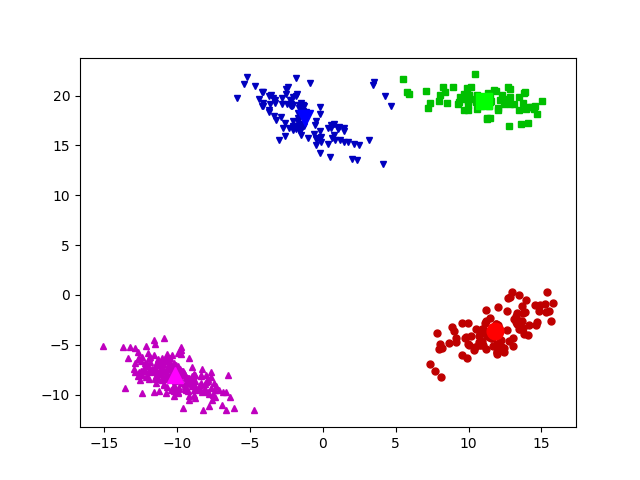
\includegraphics[width=30em]{a2_q2_1_3.png}
    \caption{Clustering with minimum error at $k=4$ (Q2.1.3)}
    \label{fig:q2_1_3}

    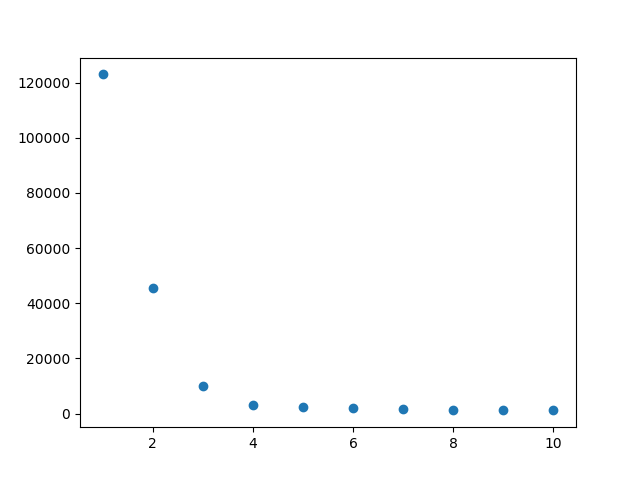
\includegraphics[width=30em]{a2_q2_2_3.png}
    \caption{Min error vs. $k$ Graph (Q2.2.3)}
    \label{fig:q2_2_3}
\end{figure}
\begin{figure}
    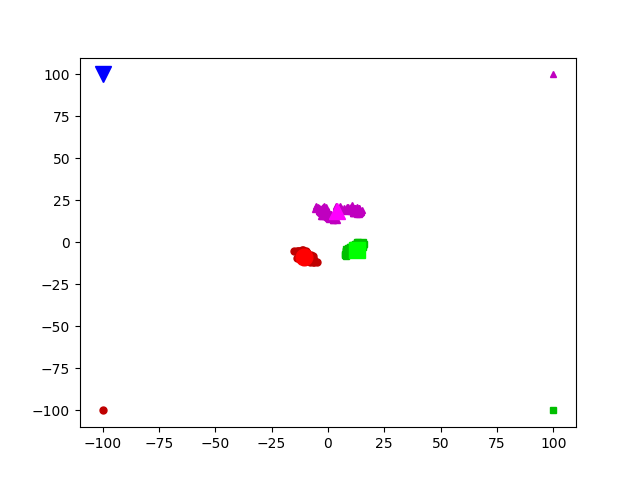
\includegraphics[width=30em]{a2_q2_3_1.png}
    \caption{Clustering with minimum error at $k=4$ (Q2.3.1)}
    \label{fig:q2_3_1}

    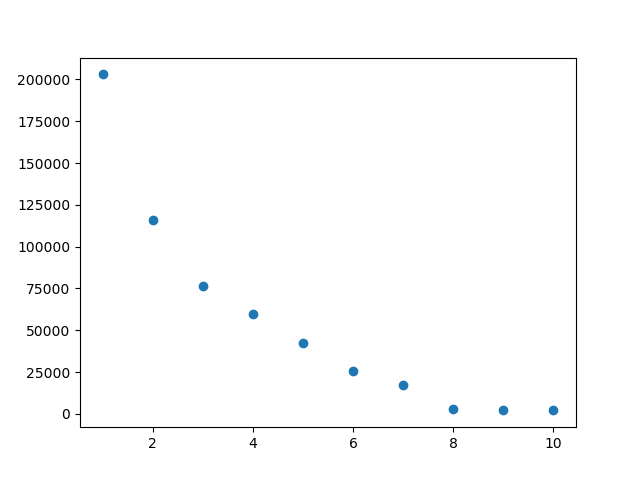
\includegraphics[width=30em]{a2_q2_3_2.png}
    \caption{Min error vs. $k$ Graph (Q2.3.2)}
    \label{fig:q2_3_2}
\end{figure}
\begin{figure}
    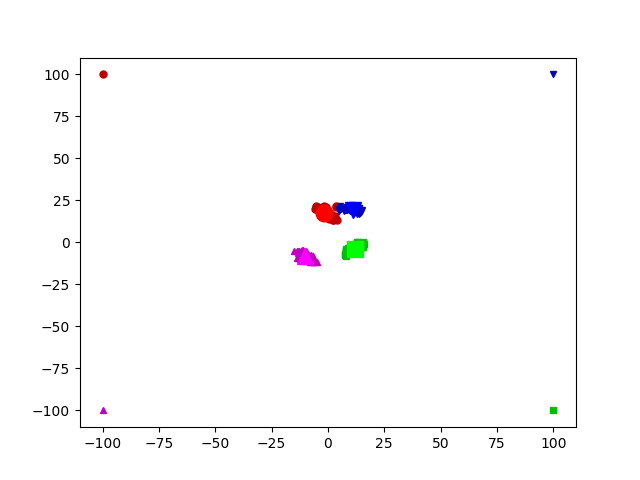
\includegraphics[width=30em]{a2_q2_3_3.png}
    \caption{Clustering of minimum error at $k=4$ (Q2.3.3)}
    \label{fig:q2_3_3}

    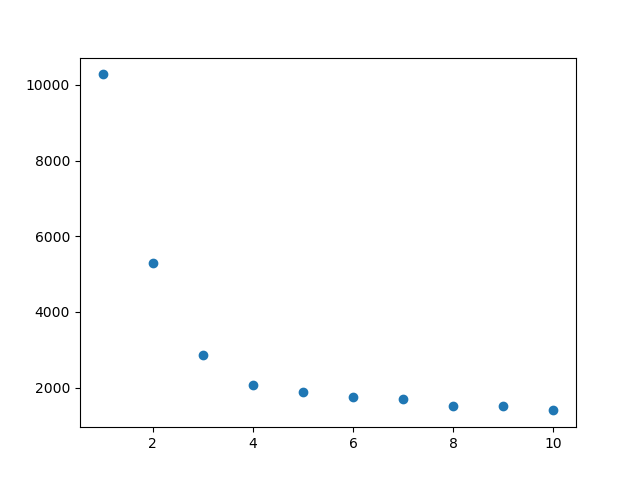
\includegraphics[width=30em]{a2_q2_3_4.png}
    \caption{Min error vs. $k$ Graph (Q2.3.4)}
    \label{fig:q2_3_4}
 \end{figure}

\section{More Unsupervised Learning}

\subsection{Density-Based Clustering}
\enum{
\item \texttt{radius = 2, minPoints = 2}
\item \texttt{radius = 4, minPoints = 2}
\item \texttt{radius = 15, minPoints = 5}
\item \texttt{radius = 50, minPoints = 2}
}

\subsection{Vector Quantization}

\begin{enumerate}
\item
\begin{verbatim}
function quantizeImage(fn,b)
    Xo = imread(fn);
    (nRows,nCols) = size(Xo);
    X = reshape(Xo, (nRows*nCols,3));

    model = kMeans(X,2^b,doPlot=false)
    return model.y,model.W,nRows,nCols
end

function deQuantizeImage(y,W,nRows,nCols)
    X = zeros(nRows*nCols,3)
    for i in 1:nRows*nCols
        X[i,:] = W[Int(y[i]),:];
    end

    Xo = reshape(X, (nRows,nCols,3));
    imshow(Xo);
    return Xo
end
\end{verbatim}
\item See Figures \ref{fig:q3_2_1}, \ref{fig:q3_2_2}, \ref{fig:q3_2_3}, \ref{fig:q3_2_4}
\end{enumerate}
\begin{figure}
    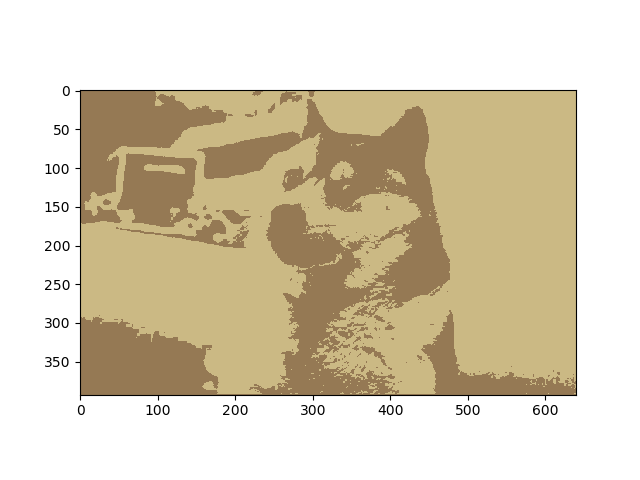
\includegraphics[width=30em]{a2_q3_2_1.png}
    \caption{dog.png encoded with 1 bit per pixel(Q.3.3)}
    \label{fig:q3_2_1}

    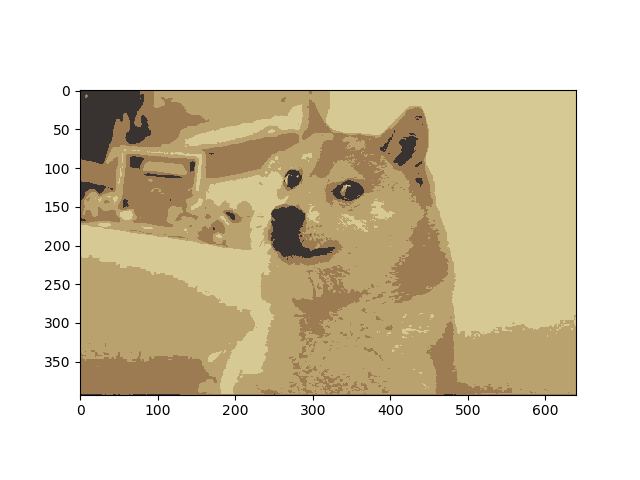
\includegraphics[width=30em]{a2_q3_2_2.png}
    \caption{dog.png encoded with 2 bits per pixel(Q3.3)}
    \label{fig:q3_2_2}
\end{figure}
\begin{figure}
    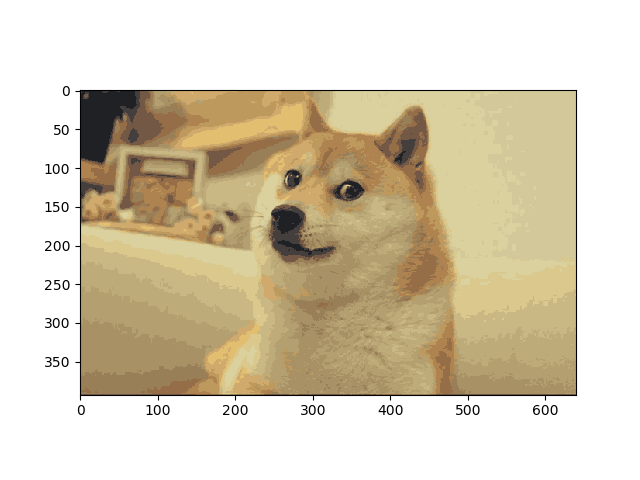
\includegraphics[width=30em]{a2_q3_2_3.png}
    \caption{dog.png encoded with 4 bits per pixel(Q3.3)}
    \label{fig:q3_2_3}

    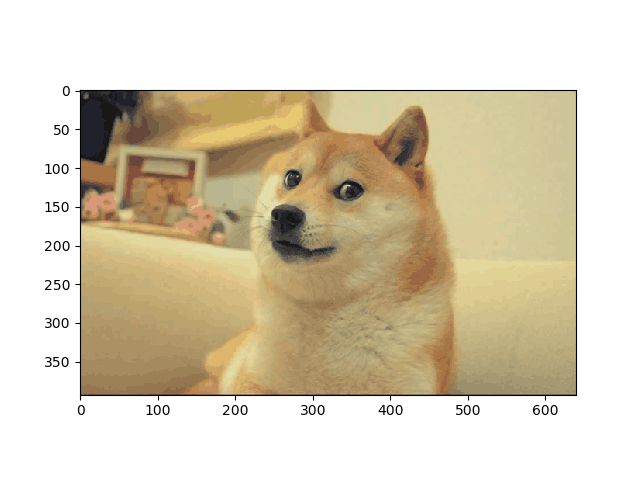
\includegraphics[width=30em]{a2_q3_2_4.png}
    \caption{dog.png encoded with 6 bits per pixel(Q3.3)}
    \label{fig:q3_2_4}
 \end{figure}
\subsection{Very-Short Answer Questions}

\enum{
\item The feature with the smaller scale would have very little influence over whether a point is 'reachable' or not. For example, a point can be very close (~1:1 ratio) to another point on the large-scale feature but very far (several times away) on the small-scale feature, but it might still be 'reachable' from the other point because the smaller-scale feature difference won't add a lot to the overall distance.
\item Advantage: we can actually tell the algorithm what is considered an 'outlier' instead of having the algorithm figure out what it is, where it may potentially be determined to be something else. Drawback: it takes a lot of time to manually label the outliers in the training dataset.
\item Essentially, we are looking for points that are within the distance $r$ from the test query point on a 2D grid. This will take $O(n)$ time because we have to go through each point. If we use the hash table approach, assuming the hash table is already filled out, this approach will require us to find the square that contains the test query and its 8 neighbors, which would take constant time since they're all stored in a hash table. Then we would have to go through the elements in each of the 9 grids to check if they are within $r$ units from the test query, so this approach will take maximum $9k$ time, i.e. $O(k)$.
}

\section{Matrix Notation and Linear Regression}

\subsection{Converting to Matrix/Vector/Norm Notation}

Using our standard supervised learning notation ($X$, $y$, $w$)
express the following functions in terms of vectors, matrices, and norms (there should be no summations or maximums).
\blu{\enum{
\item $\sum_{i=1}^n |w^Tx_i - y_i|$.
\item $\max_{i \in \{1,2,\dots,n\}} |w^Tx_i  - y_i| + \frac{\lambda}{2}\sum_{j=1}^n w_j^2$.
\item $\sum_{i=1}^n v_i (w^Tx_i - y_i)^2 + \lambda \sum_{j=1}^{d} |w_j|$.
}}
You can use $V$ to denote a diagonal matrix that has the values $v_i$ along the diagonal.

\begin{enumerate}
     \item  $ \norm{Xw-y}$
    \item  $ \norm{Xw-y}_\infty +   \frac{\lambda}{2}\norm{w}_2$
    \item  $ (Xw-y)^T V(Xw-y) +   \lambda\norm{w}_1$
 
\end{enumerate}


\subsection{Minimizing Quadratic Functions as Linear Systems}

Write finding a minimizer $w$ of the functions below as a system of linear equations (using vector/matrix notation and simplifying as much as possible). Note that all the functions below are convex  so finding a $w$ with $\nabla f(w) = 0$ is sufficient to minimiize the functions (but show your work in getting to this point).
\blu{\enum{
\item $f(w) = \frac{1}{2}\norm{w-u}^2$.
\item $f(w) = \frac{1}{2}\norm{w}^2 + w^TX^Ty$ .
\item $f(w)= \frac{1}{2}\norm{Xw - y}^2 + \frac{1}{2}w^T\Lambda w$.
\item $f(w) = \frac{1}{2}\sum_{i=1}^n v_i (w^Tx_i - y_i)^2$.
}}
Above we assume that $u$ is a $d$ by $1$ vector, and $\Lambda$ is a $d$ by $d$ diagonal matrix with positive entries along the diagonal.

Hint: Once you convert to vector/matrix notation, you can use the results from class to quickly compute these quantities term-wise. As a sanity check for your derivation, make sure that your results have the right dimensions.


\begin{enumerate}
     \item  $f(w) = \frac{1}{2}\norm{w-u}^2$\\
                      	$ = \frac{1}{2}(w-u)^T (w-u)$\\
                     	$ = \frac{1}{2}(w^T-u^T) (w-u)$\\
				$ = \frac{1}{2}(w^T w - 2w^T u + u^T u)$\\
                      	$= \frac{1}{2}\norm{w}^2 - w^T u +  \frac{1}{2}\norm{w}^2$\\
 				 $\nabla f(w) = w-u$ \\
               
    \item   $f(w) = \frac{1}{2}\norm{w}^2 + w^TX^Ty$\\
                   $ = \frac{1}{2}(w^T w) + w^TX^Ty$\\
			  $ \nabla f(w) =  w+ X^Ty$\\
   
      \item   $f(w)= \frac{1}{2}\norm{Xw - y}^2 + \frac{1}{2}w^T\Lambda w$\\
                 $= \frac{1}{2}(w^TX^T-y^T)(Xw-y) + \frac{1}{2}w^T\Lambda w$\\
			    $= \frac{1}{2}((Xw)^T(Xw)-2y(Xw)-y^Ty) + \frac{1}{2}w^T\Lambda w$\\
 			$= \frac{1}{2}w^T(x^Tx)w - w^Tx^Ty-  \frac{1}{2}y+ \frac{1}{2}w^T\Lambda w$\\
                 $ \nabla f(w) = X^TXw- X^Ty+\Lambda w$\\


        \item  $f(w) = \frac{1}{2}\sum_{i=1}^n v_i (w^Tx_i - y_i)^2$\\
                 $ = \frac{1}{2}( (Xw-y)^TV(Xw-y)$\\
                    $ = \frac{1}{2}( (w^TX^T-y^T)^V(Xw-y)$\\
                    $ = \frac{1}{2}(w^TX^TVXw - y^TVXw- w^TX^TVy+y^TVy)$\\
                     $ = \frac{1}{2}(w^TX^TVXw) -  (w^TX^TVy)+ \frac{1}{2}(y^TVy)$\\
  			$ \nabla f(w) = X^TVXw- X^TVy$\\

 
\end{enumerate}



%In class we discuss fitting a linear regression model by minimizing the squared error. 
%This classic model is the simplest version of many of the more complicated models we will discuss in the course. However, it typically performs very poorly in practice. One of the reasons it performs poorly is that it assumes that the target $y_i$ is a linear function of the features $x_i$ with an intercept of zero. This drawback can be addressed by adding a bias variable and using nonlinear bases (although nonlinear bases may increase to over-fitting). 

%In this question, you will start with a data set where least squares performs poorly. You will then explore how adding a bias variable and using nonlinear (polynomial) transforms can drastically improve the performance. You will also explore how the complexity of a basis affects both the training error and the test error. In the final part of the question, it will be up to you to design a basis with better performance than polynomial bases. If you are not familiar with Matlab, to get you started please see the notes on Matlab commands on the course webpage.

\subsection{Linear Regresion with Bias Variable}

If you run the script \emph{example\_nonLinear}, it will:
\enum{
\item Load a one-dimensional regression dataset.
\item Fit a least-squares linear regression model.
\item Report the training error.
\item Report the test error (on a dataset not used for training).
\item Draw a figure showing the training data and what the linear model looks like.
}
Unfortunately, this is an awful model of the data. The average squared training error on the data set is over 28000 (as is the test error), and the figure produced by the demo confirms that the predictions are usually nowhere near the training data:
%\centerfig{.5}{leastSquares}
The y-intercept of this data is clearly not zero (it looks like it's closer to $200$), so we should expect to improve performance by adding a \emph{bias} variable, so that our model is
\[
y_i = w^Tx_i + w_0.
\]
instead of
\[
y_i = w^Tx_i.
\]
\blu{Write a new function, \emph{leastSquaresBias}, that has the same input/model/predict format as the \emph{leastSquares} function, but that adds a \emph{bias} variable $w_0$. Hand in your new function, the updated plot, and the updated training/test error.}

Hint: recall that adding a bias $w_0$ is equivalent to adding a column of ones to the matrix $X$. Don't forget that you need to do the same transformation in the \emph{predict} function.

\begin{enumerate}


\item \begin{verbatim}

function leastSquaresBias(X,y)

     (n,)= size(X)
     X0 =  addBasis(X)
    # Find regression weights minimizing squared error
    w = (X0'*X0)\(X0'*y)

    # Make linear prediction function
    predict(Xhat) =   addBasis(Xhat)*w

    # Return model
    return GenericModel(predict)
end

function addBasis(X)
    (n,)= size(X)
    X0 = ones(n,2)
    for i in 1:n
        X0[i,2]= X[i]
     end 
   return X0
end 

 \end{verbatim}


\begin{figure}[h!]
  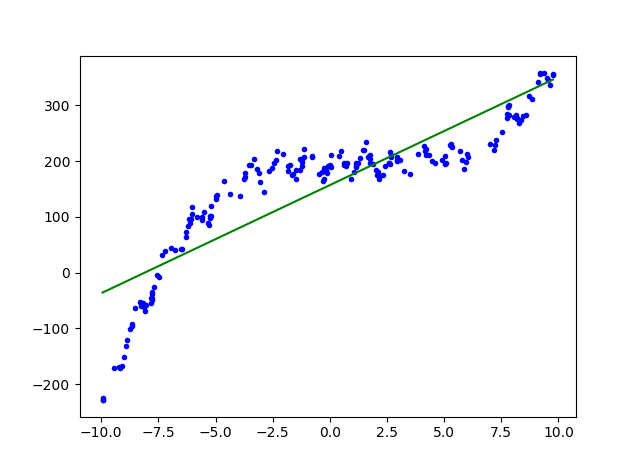
\includegraphics[width=30em,height=7.5cm]{a2_q4_3.png}

\end{figure}


\item
 \begin{verbatim}
Squared train Error with least squares: 3551.346
Squared test Error with least squares: 3393.869
 \end{verbatim}


\end{enumerate}




\subsection{Linear Regression with Polynomial Basis}

Adding a bias variable improves the prediction substantially, but the model is still problematic because the target seems to be a \emph{non-linear} function of the input. Write a new function, \emph{leastSquaresBasis(x,y,p)}, that takes a data vector $x$ (i.e., assuming we only have one feature) and the polynomial order $p$. The function should perform a least squares fit based on a matrix $Z$ where each of its rows contains the values $(x_{i})^j$ for $j=0$ up to $p$. E.g., \emph{leastSquaresBasis(x,y,3)} should form the matrix
\[
Z = 
\left[\begin{array}{cccc}
1 & x_1 & (x_1)^2 & (x_1)^3\\
1 & x_2 & (x_2)^2 & (x_2)^3\\
\vdots\\
1 & x_n & (x_n)^2 & (x_N)^3\\
\end{array}
\right],
\]
and fit a least squares model based on it.
\blu{Hand in the new function, and report the training and test error for $p = 0$ through $p= 10$. Explain the effect of $p$ on the training error and on the test error.}

Note: for this question we'll assume $d=1$ (we'll discuss polynomial bases with more input features later in the course).

Hints: To keep the code simple and reduce the chance of having errors, you may want to write a new function \emph{polyBasis} that you can use for transforming both the training and testing data. 

\begin{enumerate}
 
\item
\begin{verbatim}
function leastSquaresBasis(X,y,p)

     (n,)= size(X)
      X0 = polyBasis(X,p)


    # Find regression weights minimizing squared error
    w = (X0'*X0)\(X0'*y)

    # Make linear prediction function
    predict(Xhat) = polyBasis(Xhat,p)*w

    # Return model
    return GenericModel(predict)
end

function polyBasis(X,p)
    (n,)= size(X)
    X0 = ones(n,p+1)
    for i in 1:n
        X0[i,2]= X[i]
     end 
   for i in 3:p+1
      X0[:,i]= X0[:,2].^(i-1)
   end
   return X0
end 
 \end{verbatim}


\item
 \begin{verbatim}
Squared train Error with p: 1 and least squares: 3551.346
Squared test Error with p: 1 and least squares: 3393.869
Squared train Error with p: 2 and least squares: 2167.992
Squared test Error with p: 2 and least squares: 2480.725
Squared train Error with p: 3 and least squares: 252.046
Squared test Error with p: 3 and least squares: 242.805
Squared train Error with p: 4 and least squares: 251.462
Squared test Error with p: 4 and least squares: 242.126
Squared train Error with p: 5 and least squares: 251.143
Squared test Error with p: 5 and least squares: 239.545
Squared train Error with p: 6 and least squares: 248.583
Squared test Error with p: 6 and least squares: 246.005
Squared train Error with p: 7 and least squares: 247.011
Squared test Error with p: 7 and least squares: 242.888
Squared train Error with p: 8 and least squares: 241.306
Squared test Error with p: 8 and least squares: 245.966
Squared train Error with p: 9 and least squares: 235.762
Squared test Error with p: 9 and least squares: 259.296
Squared train Error with p: 10 and least squares: 235.074
Squared test Error with p: 10 and least squares: 256.300
 \end{verbatim}

\item As p increasing, the training error and testing error both decrease until $p$ reaches 8, at which point we start to overfit so the testing error starts to increase even as the training error goes down.

\end{enumerate}



\subsection{Manual Search for Optimal Basis}

Polynomials are a flexible class of functions, but there is structure in this data that is not well-modelled by polynomials. Try to find a nonlinear basis that gives the best performance on this dataset in terms of test error. \blu{Report the basis that you use and the training/test score that you achieve}.

Hint: the data seems to have periodic behaviour, and it's possible to obtain training and test errors below 60.

\begin{enumerate}
\item
 \begin{verbatim}

function leastTanBasis(X,y)

     (n,)= size(X)
      X0 = tanBasis(X)


    # Find regression weights minimizing squared error
    w = (X0'*X0)\(X0'*y)

    # Make linear prediction function
    predict(Xhat) = tanBasis(Xhat)*w

    # Return model
    return GenericModel(predict)
end

function tanBasis(X)
    (n,)= size(X)
    X0 = ones(n,12)

    for i in 1:n
        X0[i,2] =X[i]
        X0[i,3]= tan(0.1357*X[i])
        X0[i,4]= tan(0.1357*X[i]).^2
        X0[i,5]= tan(0.1357*X[i]).^3
        X0[i,6]= tan(0.1357*X[i]).^4
        X0[i,7]= tan(0.1357*X[i]).^5
        X0[i,8]= tan(0.1357*X[i]).^6
        X0[i,9]= tan(0.1357*X[i]).^7
        X0[i,10]= tan(0.1357*X[i]).^8
        X0[i,11] = sin(X[i])  
        X0[i,12] = sin(X[i]).^2  
         
     end 

   return X0
end

 \end{verbatim}


\item

  \begin{verbatim}
Squared train Error with least squares: 241.804 
Squared test Error with least squares: 368.812
  \end{verbatim}

\end{enumerate}

\subsection{Very-Short Answer Questions}

\blu{
\enum{
\item In this question, why are we computing the squared error $(y_i -  \hat{y}_i)^2$ and not testing the equality $(y_i = \hat{y}_i)$?
\item Describe a simple 2-feature ($d=2$) case where the least squares estimate would not be unique.
\item What is the computational complexity of computing the closed-form (exact) solution to a linear least squares problem where we have one feature ($d = 1$) and use polynomial basis of degree $p$?
\item  In what circumstance would a regression tree with linear regressions at the leaves be a better choice than a linear least squares regression model?
}}

\begin{enumerate}
\item Linear regression is usually for continuous data. It is impossible for line to pass through all the data points so testing equality would result in a practically useless and very high error. And aslo, linear regression is not predicting the exact number.
\item 
When two features that are collinear, the least squares estimate would not be unique. This is because as long as the sum of the weights of these features remains the same, we wouldn't be changing the predictions, but that also means we can change the weights in (infinitely) many was without changing the predictions, so there wouldn't be a unique minimum.

\item 
The computation needed for closed-form is \texttt{W = (X0'*X0)/(X0'*y)}. 
The runtime of  \texttt{(X0'*X0)} is $O(np^2)$, the runtime of \texttt{(X0'*y)} is $O(np)$ and  
the runtime of solving \texttt{W} is $O(p^3)$, so the total runtime  = $O(p^3) +O(np^2) + O(np)$.
Since $O(np^2)$ domidates $O(np)$ , and in generl $n>p$, therefore, total runtime = $O(np^2)$.


\item
Regression tree is suitable for data with many clusters (hard to fit one line or curve). Regression trees could split the data into different clusters and run linear regression with least squares on each cluster in the leaves as opposed to running least squares on the whole dataset.

\end{enumerate}

\section{Robust Regression and Gradient Descent}

The script \emph{example\_outliers} loads a one-dimensional regression dataset that has a non-trivial number of `outlier' data points. These points do not fit the general trend of the rest of the data, and pull the least squares model away from the main downward trend that most data points exhibit:
%\centerfig{.7}{outliers}




\subsection{Weighted Least Squares in One Dimension}

One of the most common variations on least squares is \emph{weighted} least squares. In this formulation, we have a weight $v_i$ for every training example. To fit the model, we minimize the weighted squared error,
\[
f(w) =  \frac{1}{2}\sum_{i=1}^n v_i(w^Tx_i - y_i)^2.
\]
In this formulation, the model focuses on making the error small for examples $i$ where $v_i$ is high. Similarly, if $v_i$ is low then the model allows a larger error.

Write a model function, \emph{weightedLeastSquares(X,y,v)}, that implements this model (note that a previous question asks you to show how this formulation can be solved as a linear system).
Apply this model to the data containing outliers, setting $v_i = 1$ for the first $400$ data points and $v_i = 0.1$ for the last $100$ data points (which are the outliers). \blu{Hand in your function and the updated plot}.


  \begin{verbatim}

function weigthedleastSquares(X,y,v)
    (n,) = size(v)
    V =  zeros(n,n)
     
    for i in 1:n
        for j in 1:n
            if i==j
                V[i,j]=v[i]
              end 
        end
    end
    
    w = (X'*V*X)\(X'*V*y)
    # Make linear prediction function
    predict(Xhat) = Xhat*w

    # Return model
    return GenericModel(predict)
end

  \end{verbatim}

\begin{figure}[h!]
  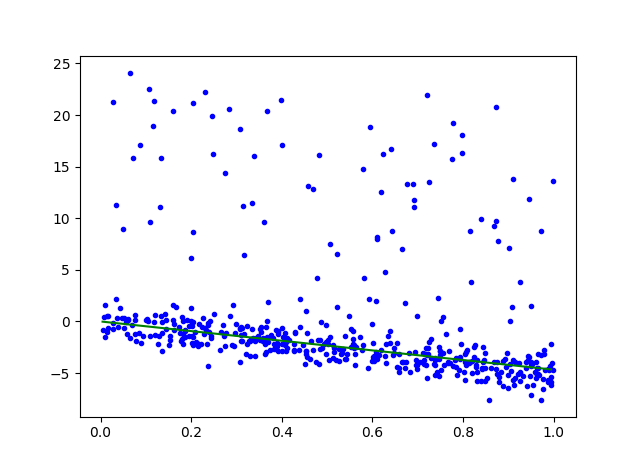
\includegraphics[width=30em,height=7.5cm]{a2_q5_1.png}

\end{figure}



\subsection{Smooth Approximation to the L1-Norm}

Unfortunately, we typically do not know the identities of the outliers. In situations where we suspect that there are outliers, but we do not know which examples are outliers, it makes sense to use a loss function that is more robust to outliers. In class, we discussed using the sum of absolute values objective,
\[
f(w) = \sum_{i=1}^n |w^Tx_i - y_i|.
\]
This is less sensitive to outliers than least squares, but it is non-differentiable and harder to optimize. Nevertheless, there are various smooth approximations to the absolute value function that are easy to optimize. One possible approximation is to use the log-sum-exp approximation of the max function\footnote{Other possibilities are the Huber loss, $|r| \approx \sqrt{r^2 + \epsilon}$ for some small $\epsilon$.}
\[
|r| \approx \log(\exp(r) + \exp(-r)).
\]
%for some parameter $\alpha$. This approximation becomes exact as $\alpha$ goes to $\infty$, but for any fixed $\alpha$ the function will be differentiable.
Using this approximation, we obtain an objective of the form
\[
f(w) = \sum_{i=1}^n  \log\left(\exp(w^Tx_i - y_i) + \exp(y_i - w^Tx_i)\right).
\]
which is smooth but less sensitive to outliers than the squared error. \blu{Derive
 the gradient $\nabla f$ of this function with respect to $w$. You should show your work but you do not have to express the final result in matrix notation.}

$\nabla _w(log(exp(w^Tx_i-y_i)+exp(y_i-w^Tx_i))= \frac{x_i(exp(w^Tx_i-y_i)-exp(y_i-w^Tx_i))}{(exp(w^Tx_i-y_i)+exp(y_i-w^Tx_i))ln(e)}$\\
$\nabla f= \sum\limits_{i=1}^{n}\frac{x_i(exp(w^Tx_i-y_i)-exp(y_i-w^Tx_i))}{(exp(w^Tx_i-y_i)+exp(y_i-w^Tx_i))}$

\subsection{Robust Regression}

The function \emph{example\_gradient} is the same as \emph{example\_outlier}, except that it fits the least squares model using a \emph{gradient descent} method. You'll see that it produces the same fit as we obtained using the normal equations.
%One advantage of this strategy is that it only costs $O(nd)$ for an iteration of the gradient method, which is faster than forming $X^TX$ which costs $O(nd^2)$. Of course, we need to know the \emph{number} of gradient iterations in order to precisely compare these two strategies, but for now we will assume that the number of gradient iterations is typically often reasonable.

The typical input to a gradient method is a function that, given $w$, returns $f(w)$ and $\nabla f(w)$. See \emph{funObj} in the \emph{leastSquaresGradient} function for an example. Note that \emph{leastSquaresGradient} also has a numerical check that the gradient code is approximately correct, since implementing gradients is often error-prone.\footnote{Though sometimes the numerical gradient checker itself can be wrong. For a lot more on numerical differentiation you can take CPSC 303.}

An advantage of gradient-based strategies is that they are able to solve problems that do not have closed-form solutions, such as the formulation from the previous section. The function \emph{robustRegression} has most of the implementation of a gradient-based strategy for fitting the robust regression model under the log-sum-exp approximation. The only part missing is the function and gradient calculation inside the \emph{funObj} code. \blu{Modify this function to implement the objective function and gradient based on the smooth approximation to the absolute value function (from the previous section). Hand in your code, as well as the plot obtained using this robust regression appraoch.}

\begin{enumerate}

\begin{figure}[h!]
  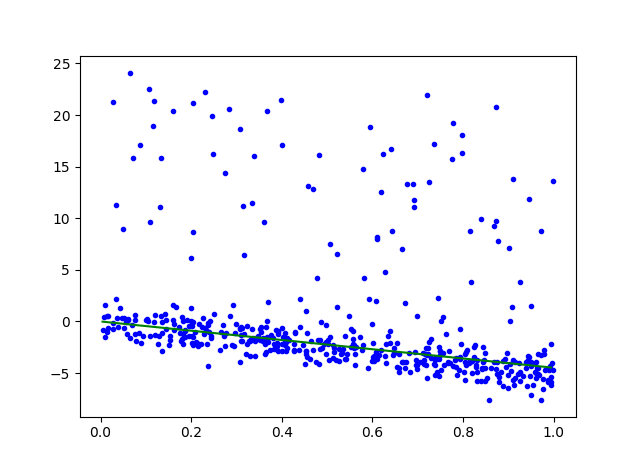
\includegraphics[width=30em,height=7.5cm]{a2_q5_3.png}

\end{figure}

\item
  \begin{verbatim}
function leastSquaresObj(w,X,y)
    f = sum(log(exp.(X*w-y)+exp.(y-X*w)))
    g = X'*((exp.(X*w-y)-exp.(y-X*w))./(exp.(X*w-y)+exp.(y-X*w)))
    return (f,g)
end

  \end{verbatim}

\end{enumerate}

\subsection{Very-Short Answer Questions}

\enum{
\item 1. Graph-based: this would be effective for this dataset because the dataset is in 2D, which means it's easy to make into a human readable graph. And from the graph we can easily tell where the outliers are in a very short amount of time. Even though labelling might take a while, this data set is relatively small so it's definitely doable. 2. Model-based: it won't work as well because the mean and variance are sensitive to outliers, which we have a lot here. If we use this approach, the mean would likely end up somewhere close to the middle, which means it will only detect some of the outliers at the top but likely not the ones closer to the middle.
\item When $d$ (number of features) gets too large. This is because the closed form solution takes $O(nd^2+d^3)$ time, so it scales up very quickly as $d$ goes up, due to the squares and cubes, whereas gradient descent takes $O(ndt)$ time so it doesn't scale up as much.
\item The absolute value graph may not have a point where gradient is 0, as it keeps going down and then back up again in a sharp corner. Due to the discontinuity the gradient at the minimum may actually be undefined so cannot be solved by the gradient method. If we smooth the absolute value though, the sharp corner goes away and the function becomes continuous, which means we can actually find the local min with gradient descent.
}


\begin{enumerate}
\item  Clusterbased
\item
\begin{verbatim}
  The runtime of closed form is  O(nd^2 +d^3). And the runtime of gradient descent is O(nd). we should consider it when D is large. 
  \end{verbatim}
\item Because there are a lot linear systems that we cannot easy to solve it.   

\end{enumerate}
\end{document}